%%% Fiktivní kapitola s ukázkami citací


\chapter{Kalibrace kamery}
Kalibrace kamery znamená nalezení jejich vnitřních a vnějších parametrů.
Slouží v počítačovém vidění pro skládání obrazu z více snímků nebo pro vytváření 3D modelů.


Kalibrace kamery se dá provádět s nebo bez pomoci snímků, na nichž se nachází známé kalibrační objekty.
V této kapitole se zaměříme na srovnání dvou odlišných metod kalibrace kamery a to na \cite{Lalonde10} a \cite{deepcalib}, které nevyžadují kalibrační objekty.
\section{Zdrojová data}
Práce využívá obrazových dat z veřejně dostupných webových meteorologických kamer Českého hydrometeorologického ústavu (ČHMÚ).


\begin{figure}[h]\centering
    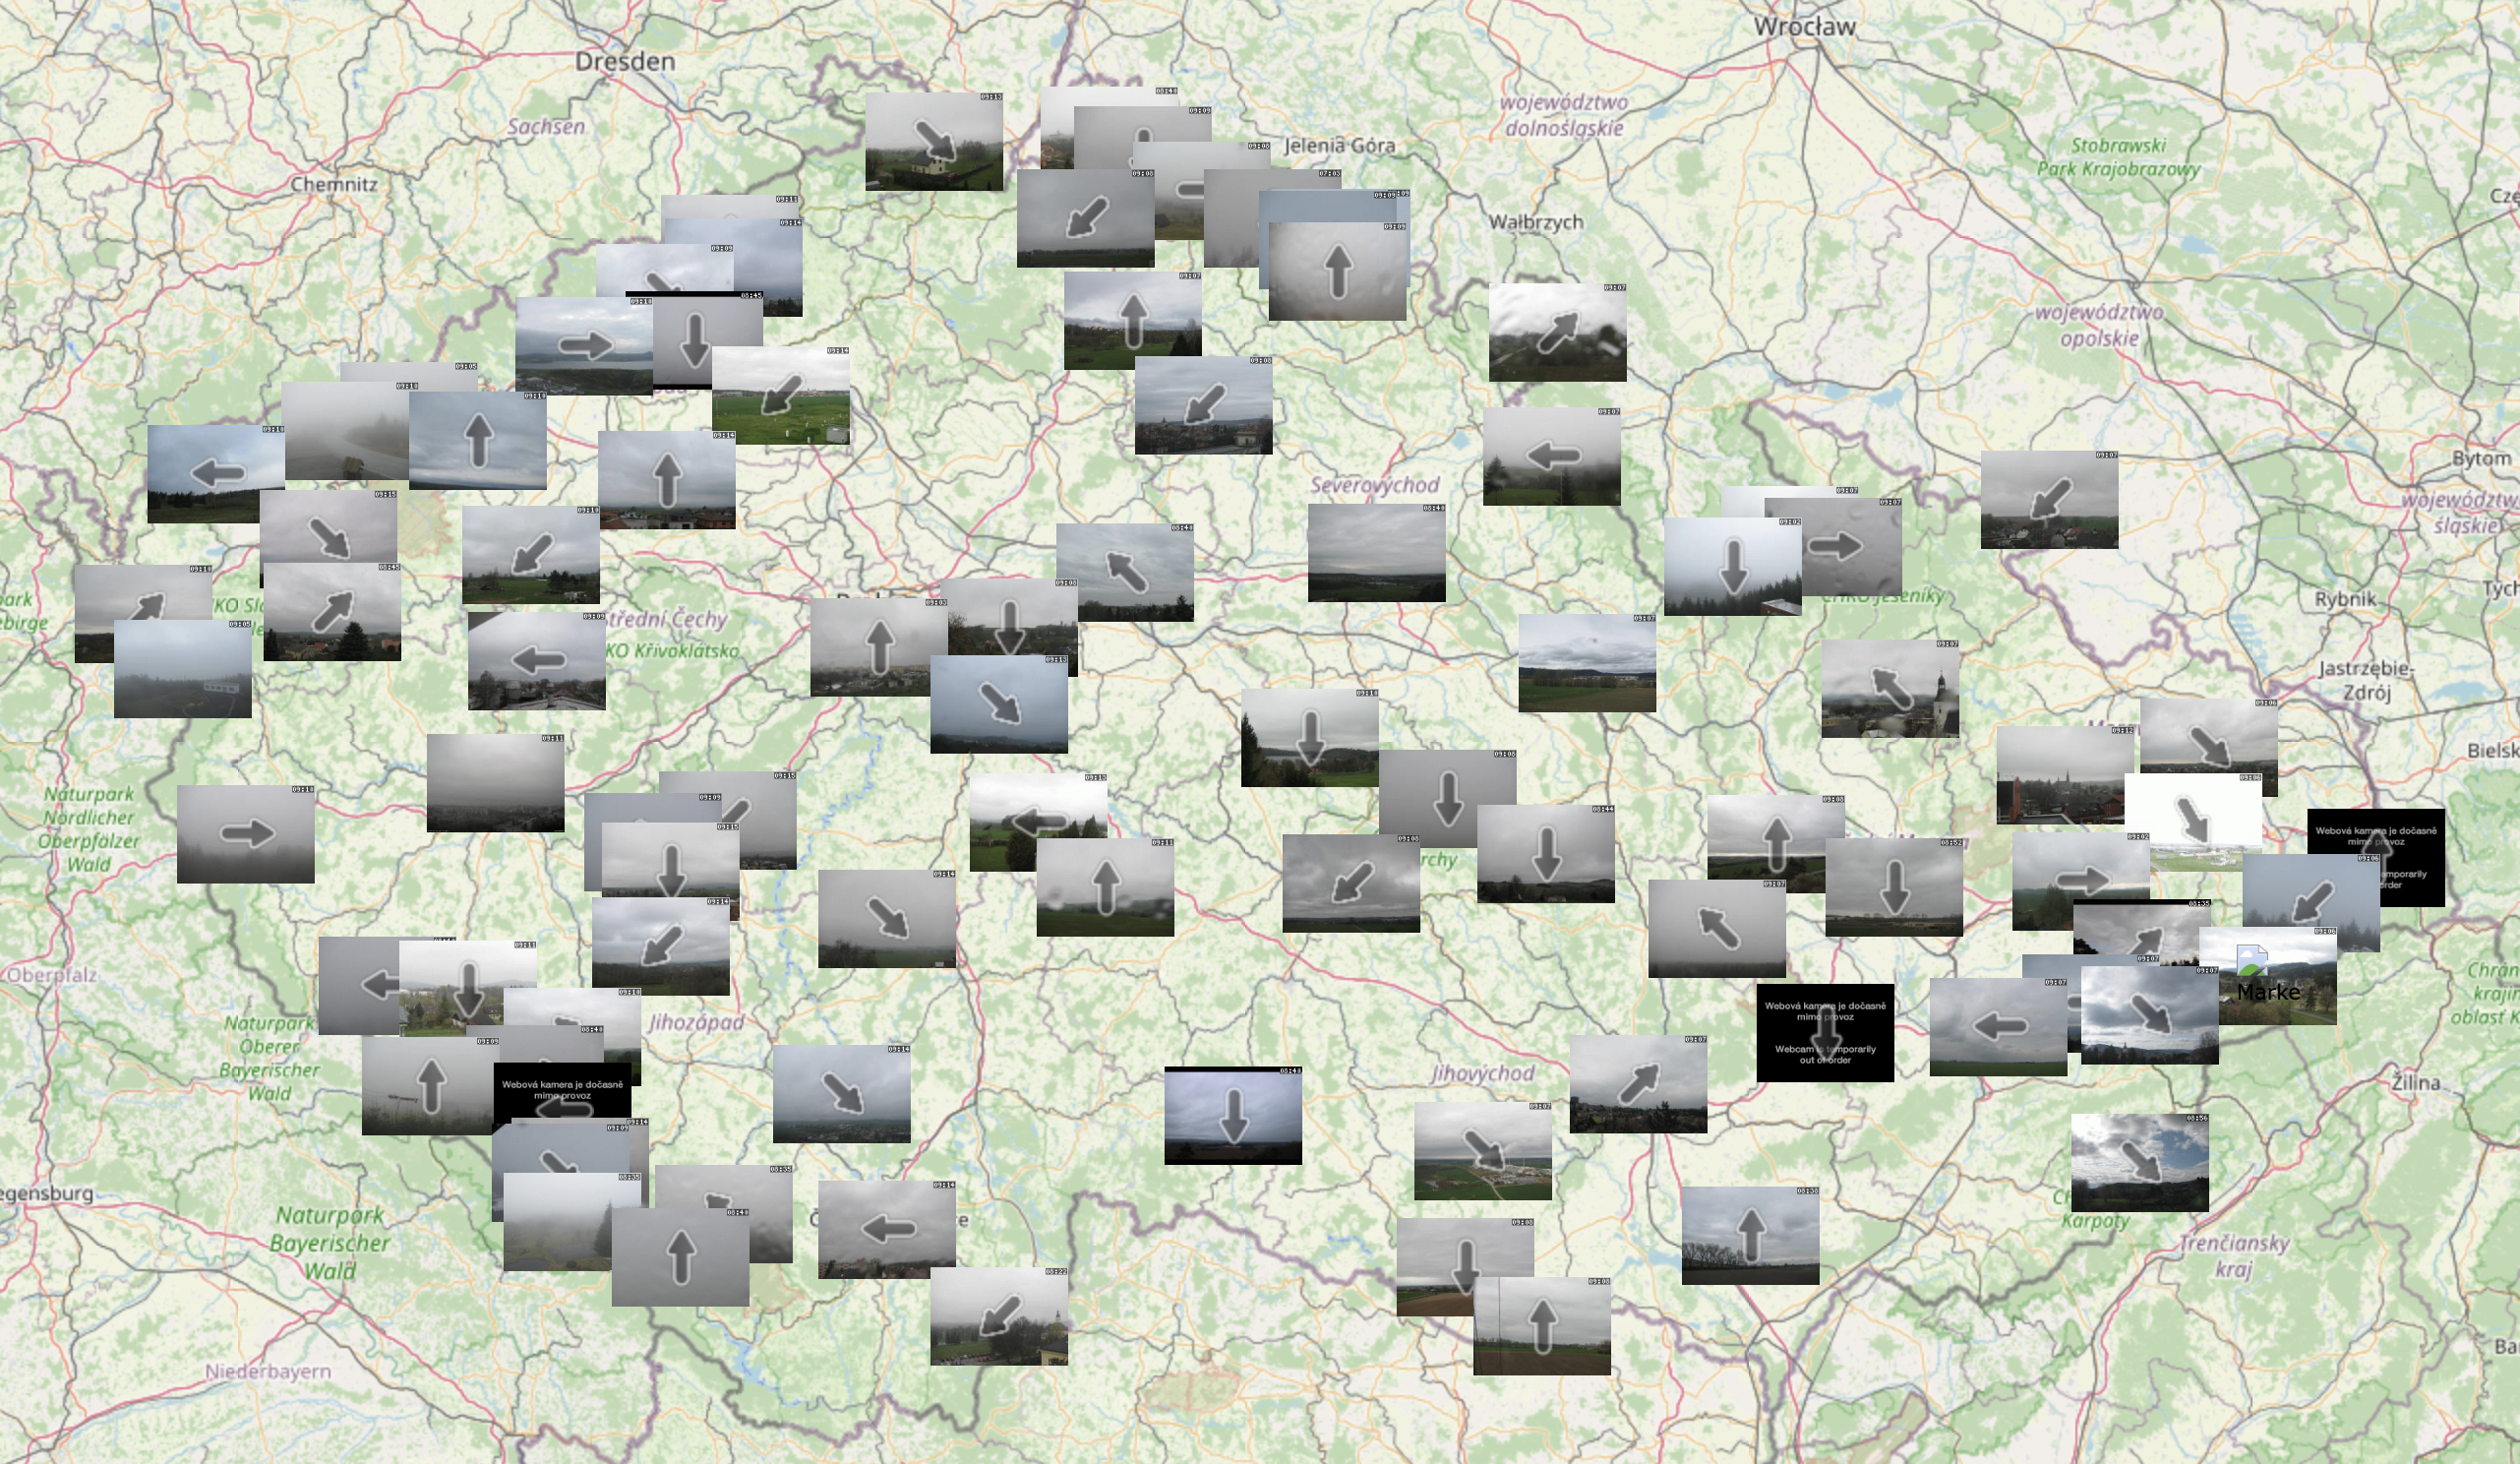
\includegraphics[width=140mm]{../img/map}
    \caption{Mapa webových kamer \cite{chmu}}

\end{figure}

\section{Příprava datasetu}


\section{Co dělá Lalonde TODO}
